
 
\documentclass[11pt]{article}
\addtolength{\oddsidemargin}{-1.cm}
\addtolength{\textwidth}{2cm}
\addtolength{\topmargin}{-2cm}
\addtolength{\textheight}{3.5cm}
\newcommand\tab[1][1cm]{\hspace*{#1}}
\usepackage[pdftex]{graphicx}
\usepackage{pdflscape}
\usepackage{hyperref}
\usepackage[T1]{fontenc}
\usepackage{float}
\usepackage{cite}
\hypersetup{
	colorlinks=true,
	linkcolor=black,
	filecolor=magenta,
	urlcolor=cyan,
}

% define the title
\author{Panda Inc}
\title{Multiply Active-Days}
\begin{document}
\begin{titlepage}
	
	\begin{center}
		% Upper part of the page         
        
\includegraphics[width=0.7\linewidth]{PandaInc_logo.jpg}\\[1cm] 
		\textsc{\LARGE Panda Inc}\\[0.3cm]
		% Title
		\rule{\linewidth}{0.5mm} \\[1cm]
		{ \huge \bfseries  System Requirements Specification}\\[0.5cm]
		\rule{\linewidth}{0.5mm} \\[1cm] 		
  
		
		\begin{minipage}{0.4\textwidth}
			\begin{flushleft} \large
				\emph{} \\
				Quinton {Swanepoel}
			\end{flushleft}
		\end{minipage}
		\begin{minipage}{0.4\textwidth}
			\begin{flushright} \large
				\emph{} \\
				15245510
			\end{flushright}
		\end{minipage}

		\begin{minipage}{0.4\textwidth}
			\begin{flushleft} \large
            	\emph{} \\
				Azhar {Patel}
			\end{flushleft}
		\end{minipage}
		\begin{minipage}{0.4\textwidth}
			\begin{flushright} \large
				\emph{} \\
				15052592
			\end{flushright}
		\end{minipage}
		
		\begin{minipage}{0.4\textwidth}
			\begin{flushleft} \large
				\emph{} \\
				Tshepo Macebo {Malesela}
			\end{flushleft}
		\end{minipage}
		\begin{minipage}{0.4\textwidth}
			\begin{flushright} \large
				\emph{} \\
				14211582
			\end{flushright}
		\end{minipage}

		\begin{minipage}{0.4\textwidth}
			\begin{flushleft} \large
				\emph{} \\
				Monkeli Fred {Dilapisho}
			\end{flushleft}
		\end{minipage}
		\begin{minipage}{0.4\textwidth}
			\begin{flushright} \large
				\emph{} \\
				15074260
			\end{flushright}
		\end{minipage}
        
        \begin{minipage}{0.4\textwidth}
			\begin{flushleft} \large
				\emph{} \\
				Keaton {Pennels}
			\end{flushleft}
		\end{minipage}
		\begin{minipage}{0.4\textwidth}
			\begin{flushright} \large
				\emph{} \\
				14373018
			\end{flushright}
		\end{minipage}
		
		\rule{\linewidth}{0.5mm} \\[1cm] 
		\textsc{\Large Stakeholders}\\[1cm]	
		
		\begin{minipage}{0.4\textwidth}
			\begin{flushleft} \large
				\emph{} \\
				Multiply:
			\end{flushleft}
		\end{minipage}
		\begin{minipage}{0.4\textwidth}
			\begin{flushright} \large
				\emph{} \\
				Philip Kruger
			\end{flushright}
		\end{minipage}

		
	\end{center}
\end{titlepage}

\newpage
\tableofcontents
\section{Introduction}
The section gives an overall description and overview of the system and the SRS document. The purpose for the document will be described and helpers such as abbreviations and definitions will be provided.
\subsection{Purpose}
The purpose of this software requirements specification document is to give detailed descriptions, the systems requirements and the systems constraints for the Momentum Multiply Active days application. The application interfaces, behaviors and interactions with other applications which includes the mobile application, server communication and the web interface.
\subsection{Project Scope}
The main purpose of this system is monitor or track Multiply members when they visit Multiply partners or particular events or areas. The system will keep track of where and how many times a user has visited these locations and report the data back to the server where it will be stored. Based on the time spent at these locations the user will receive points called 'ActiveDays'. These points will be summed up for a reward policy for the user and the more 'ActiveDays' the better they chances of getting more rewards. 
\subsection{Definitions,Acronyms and Abbreviations}
\textbf{R1,R2, R\textit{N}} specifies a requirement \\
\textbf{UC1,UC2, UC\textit{N}} specifies a use case \\
\textbf{DC1, DC2, DC\textit{N}} specifies a design constraint
\textbf{User} - A Momentum Multiply registered account holder\\
\textbf{Administrator} - A user that monitors the system and does maintenance too.
\subsection{References}
[1] David C. Kung "Object-Oriented Software Engineering, An Agile Unified Methodology", 2014.
\subsection{Overview}
The remainder of this document will include three sections that will be organized as follows:
Section two will describe the Background, which includes the business/research opportunity to
simplify the Multiply ActiveDays Application, the administration and management of users and beacons for the application. This section also sheds light on the problems being faced that may have led
to this project being started. The following section will be the Overall Description, this section basically explains what the client wants to achieve with the project and what the average user would get out of the Application. The final section will be the Specification Requirements, which will capture the functionality which would be required by users of the system.
\subsection{Background}
The main purpose of the system is to provide a means for Multiply clients to get credited for time spent with Multiply partners. The systems Mobile application allows for the monitoring of time spent with Multiply partners. The Mobile application provides a method for the users to view the points that they have accumulated called 'ActiveDays', this will be based on the Multiply algorithms and the time monitored by the application, there are other factors but are not relevant to this project.\\
The Mobile application will also give user notifications when in an area of concern, the user will receive a  push notification with some of the Multiply partner's details such as name and location. \\
The system also provides a method for managing the mobile application users and the beacons, the administration of the system will be provided by a web interface that will contain function necessary for user and beacon management, these include CRUD operations of users and beacons.\\
\section{Overall Description}
In this section we give an overview of the system and also provide some detail on how the system interacts with the components or subsystems in uses. This section will also describe basic functionality that the system will provide. The use of the system by the different types of users mainly users, administrators, and partners.     
\subsection{Product Perspective}
The Momentum Multiply ActiveDays system consists mainly of four parts, these are the mobile application, the administrator web interface, the beacons and the cloud based server. The mobile application will be used by the users of the system to monitor their time and attendance at Multiply partners locations. The web interface will be used by the administrator to manage the users, partner, locations and number of beacons at the location, and other functionality. The beacons will be used to register users to a location and monitor the time they spend at that particular location. The server will be used to grant access to the application for the users, it also waits for user data from the users mobile application to register where and how long the user was at a location.\\\\
The mobile application will alert the user when they enter a location with a Multiply partner, in the background the application will monitor the time spent by the user at the particular locations. The mobile application uses bluetooth to communicate with the beacons and when the device is within range the user should get an alert informing them of the Multiply partner location they have entered. The mobile application will also communicate with the server to report the time and the location visited. \\\\
The beacons will be be registered to a Multiply partner and will communicate with the mobile application of the user. Each beacon will have a unique identification to differentiate the different locations and the partner. Since Multiply partner may have more than one beacon registered to them, an identification method for the partner will be on the beacons.\\\\
\subsubsection{System Interfaces}
The  system interface will include the communication of the mobile device and the server, the web device and the server, and the mobile device and the beacons. 
Both the web interface and the  mobile application will require the use of similar services from the, server. The mobile application will be used for services such as user validation and authentication, retrieving user charts for the leaders board and the communities within the application. The web interface will also share certain  method requests from the server as the mobile application, these would be the get user(s) to view and perform operations on the users and, the web interface will also support services for beacon management. \\
The user data will be retrieved from the Multiply user database, this data will be stored in our database and be used as reference to the users in order to not affect Multiply data. Our server will communicate with the multiply server to exchange user data. Our data records will have an extra field for application activation called 'active' to signify that the user has or has not registered the application, and 'active' field the user will or will not be granted use of the mobile application. The system will store all users including the ones that no long use the system for future lookups, and in case the user returns to the application and require they data. \\
In the web interface all the user activity will be visible but un-editable, the administrator has the ability user events, view the user profile and delete the user if need be. \\
The web interface will also have functionality to add, remove and edit beacons registered to Multiply Partners, these will be the beacons use by the Multiply partners and these are the same beacons that will register a user at a location. When the user mobile devices sends data to the server to store an event, it will send a particular beacon id used to register the beacon to the location.\\ 
\subsubsection{User Interfaces}
The first thing a first-time user of the mobile application will see after opening the application is a login screen. If the user has not registered the application they should be able to do so on the login screen. For non-first-time users, the user will see a profile page.\\
In the profile page, the user can view details of their ActiveDays and profile information. There will also be a sign-out option on the page if the user wants to log out.\\
When a user enters a Multiply partners location, they should have some sort of alert or notification that when opened, the application will show the location visited and the partner visited and maybe some details of the location.
There will be a login for the web application, it will be simple and ask for a user-name and password. Once an administrator has logged in, they will see have a drawer containing the available sections that they can select. These sections will relate to the user and beacon management settings. Depending on which section the administrator chooses the page will navigate to the section but the drawer will still be available.
\subsubsection{Hardware Interfaces}
The web application will not use any dedicated hardware therefore there is no hardware interface for the web application.The mobile application however does have a hardware interface, beacons are basically dedicated hardware devices to aid the mobile applications ability to detect location and presence. The mobile application will use the device's blue-tooth to connect to the beacons, the beacon devices will always be waiting for a connection and when the mobile device is in range, the connection should be established. For this to happen, the mobile devices blue-tooth has to be enable before entering the location of  Multiply partner, if not there will be no connection thus removing the system functionality.
\subsubsection{Software Interfaces}
The mobile application communicates with two entities, the cloud based server and the beacons. The mobile device communicates to the beacons to allow for the location of the device to be known and for how long the device is in the particular location. The beacons have a range which once a mobile device is within, the connection is established. The mobile application also communicates with the server to write data about the time spent at a particular location to the database, requests for user data and other data services relevant to the user from the database.
The web interface communicate with the server to request database services to read, modify and create new data on users and beacons. 
\subsubsection{Communication Interface}
Communication between the various components of the system is very important. The web web interface will use HTTP/HTTPS protocol to communicate over the Internet. The mobile application will also use HTTP to communicate over the Internet. The mobile  application will also use blue-tooth to communicate with the beacons.
\subsubsection{Memory}

\subsubsection{Operations}
For this section the operations performed by the mobile application and the web interface. \\
For the mobile application, the first operation is the user registration and user login, these operations will verify the user by sending a REST API request to the server to authenticate the user.
Once the user has logged in they will have the ability to perform actions that will enable then to:-
\begin{itemize}
	\item View their accumulated active days
	\item View leader-boards.
	\item View your community and global communities. 
	\item Join communities.
	\item Create communities
	\item Challenge communities.
	\item Invite friends to a community
	\item Tap to share achievements to social media.
	\item View user data.
\end{itemize}
The web interface will also share the same first operation as the mobile application which is user registration and authentication.\\
The operations that can be performed on the web interface include:
\begin{itemize}
	\item View all active users (i.e users registered to use the application)
	\item View single user
	\item Remove/deactivate user.
	\item View user events and records.
	\item Add new beacon to new location or location that already exists on the system
	\item Change beacon registration location.
	\item Remove beacons from a location.
\end{itemize}
\subsubsection{Site Adaptations Requirements}

\subsection{Product Functions}
The administrative web portal will varies functions, these include create/granting users permission to use the application, removing users from being able to access the application. The administrator can also view all users currently on the system. The administrative web portal also has a beacon management module that allows for addition of beacons, editing of a beacon's registration details and removing beacons from locations.  The administrative web portal also has functionality to edit admin settings. An Extra functionality for the administrator is to be able to send notifications directly from the web portal to a selective set of users on the mobile application. \\
The mobile application will also have varies functions, the main function of the application is monitor user activity around Multiply partners, this will require the user to accept the use of blue-tooth by the application. \\  
The mobile application also has a method for getting the number of active days there are, this will be generated based on the number of days the application has monitored you around Multiply partners.  There will be functions to join communities and view leader-boards as a form of gamification. The mobile application also has the functions to create or join challenges.  
\subsection{User Characteristics}
There will be two main users that interact and communicate with the system, the mobile application users and the administrator users. Both of these users communicate and interact with the system in different ways, the mobile application users use the application to monitor the attendance at Multiply partner location, and see user data. The administrative user uses the web interface to perform beacon management and user management functions. These services include CRUD operations on both users and beacons.
   
\subsection{Constraints}
The mobile application is constrained by the time to check of the blue-tooth connection, as these will not be the same for each mobile device and therefore there might be seconds elapse from the calculated time spent at a location.\\
The mobile application will have to be able to communicate with the server meaning there has to be a reliable Internet connection, this may be a constraint for  users who run out of data, this can be resolved by keeping the data until there is a connection available.\\
\subsection{Assumptions and Dependencies}
\begin{itemize}	
	\item User has active Internet connection. 
	\item User's mobile device has blue-tooth.
	\item User's mobile application is Android	
\end{itemize}
\section{Specific Requirements}
\subsection{External Interface Requirements}
\subsection{Functional Requirements}
\textbf{R1}The users must be able to download the application via a mobile application store or any other similar service.\\
\textbf{R2}User Registration
\begin{itemize}	
	\item \textbf{R2.1}Only users that are registered to the Momentum Multiply database can have register and login to the application.
	\item \textbf{R2.2}Users will be asked to register the application with they Multiply user name and password, which will then be validated.
\end{itemize}
\textbf{R3} Beacon Management
\begin{itemize}	
	\item \textbf{R3.1}Each beacon must be registered to Multiply participating partner.
	\item 	\textbf{R3.2}There can be more than one beacon in a particular location provided the beacons are registered to the same Multiply participating partner.
	\item \textbf{R3.3} The system has to have an identifier for beacons that belong to the same partner and beacons belonging to different partners.	
\end{itemize}
\textbf{R4} User Management
\begin{itemize}	
	\item \textbf{R4.1}Users will register the application with they Multiply user name and password, all users who register will be must be on the existing Multiply Database. 
	\item \textbf{R4.2} The administrator can perform CRUD operation on the users and user data. 
	\item \textbf{R4.3}A Lookup on where and which locations the users where present can be performed.
	 deactivate 
\end{itemize}
\textbf{R5} The system Administrator should have access to a web portal where they will do user and beacon management. \\
\textbf{R6} The mobile device must track whenever a user is within the space of a partner, i.e the user must be notified when around a partner. \\
\textbf{R7} The mobile application must give notifications to the users when the user is around a nearby partner. \\
\textbf{R8} The mobile application will record the time and track all partner locations visited. \\
\textbf{R9} The mobile application will have a community where users can compete and interact with one another..\\
\textbf{R10} A leader-board will be available on the mobile application or users to compete with one another.  \\
\textbf{R11} The user has the ability to request an active day based on their use of the application.
\begin{itemize}	
	\item \textbf{R11.1}The active day is calculated on the server, based on the time spent by the user at partner locations.
	\item \textbf{R11.2}The user is only allowed to request one active day a day. 	
\end{itemize}
\subsubsection{Use Cases/Service Contract}
\textbf{UC1 Download Application}\\
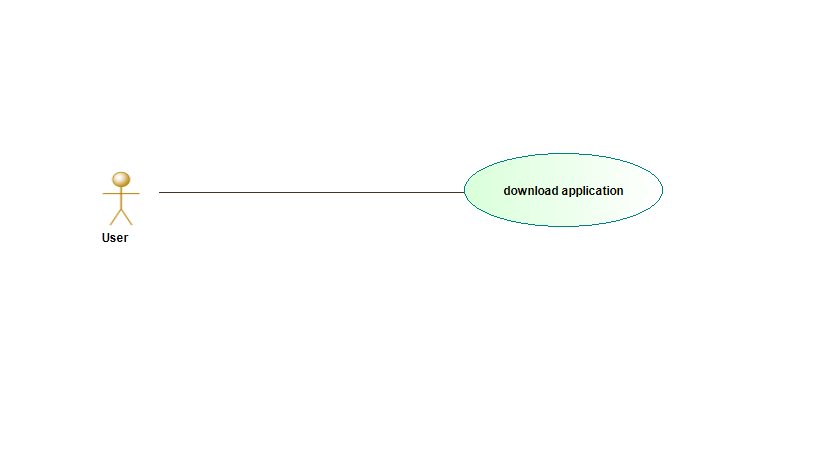
\includegraphics[scale=0.5]{./DiagramsTshepo/downloadApp.png}\\
\textbf{Pre-condition: }   \\
\begin{itemize}
	\item The user must own a android device
	\item The user must have a Internet connection.
\end{itemize}
\begin{center}
	\begin{tabular}{ |p{8cm}|p{8cm}| }
		\hline
		\textbf{Actor:} User & \textbf{System:} ActiveDays \\
		\hline
		  &  \\
		\hline
		 &  \\
		\hline
		 & \\   
		\hline
		  & \\
		\hline
	\end{tabular}
\end{center}		
\textbf{Post-condition: } \\
\begin{itemize}
	\item The Multiply Active Days mobile application will be downloaded onto you mobile device.
\end{itemize}	
\textbf{UC2 Application Community}\\\\
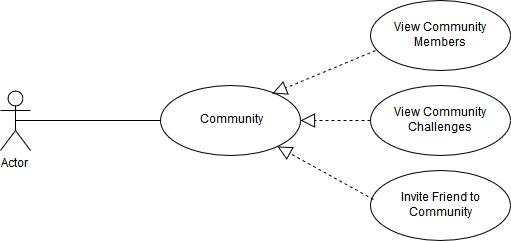
\includegraphics[scale=0.5]{./DiagramsAzhar/Community1.png}\\\\
\textbf{Pre-condition: }   \\
\begin{itemize}
	\item User need to be registered as Multiply application user.
	\item The user must have a Internet connection.
\end{itemize}
\begin{center}
	\begin{tabular}{ |p{8cm}|p{8cm}| }
		\hline
		\textbf{Actor:} User & \textbf{System:} ActiveDays \\
		\hline
		&  \\
		\hline
		&  \\
		\hline
		& \\   
		\hline
		& \\
		\hline
	\end{tabular}
\end{center}		
\textbf{Post-condition: } \\
\begin{itemize}
	\item Users can view Communities on the application
\end{itemize}	
\textbf{UC3 Application Challenges}\\\\
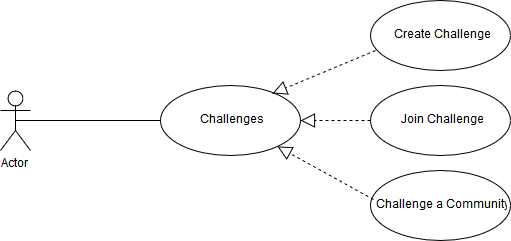
\includegraphics[scale=0.5]{./DiagramsAzhar/Community2.png}\\\\
\textbf{Pre-condition: }   \\
\begin{itemize}
	\item User need to be registered as Multiply application user
	\item The user must have a Internet connection.
\end{itemize}
\begin{center}
	\begin{tabular}{ |p{8cm}|p{8cm}| }
		\hline
		\textbf{Actor:} User & \textbf{System:} ActiveDays \\
		\hline
		&  \\
		\hline
		&  \\
		\hline
		& \\   
		\hline
		& \\
		\hline
	\end{tabular}
\end{center}		
\textbf{Post-condition: } \\
\begin{itemize}
	\item 
\end{itemize}
\textbf{UC4 Application Leadership}\\\\
\includegraphics[scale=0.5]{./DiagramsAzhar/LeaderBoard.png}\\\\

\textbf{Pre-condition: }   \\
\begin{itemize}
	\item User need to be registered as Multiply application user
	\item The user must have a Internet connection.
\end{itemize}
\begin{center}
	\begin{tabular}{ |p{8cm}|p{8cm}| }
		\hline
		\textbf{Actor:} User & \textbf{System:} ActiveDays \\
		\hline
		&  \\
		\hline
		&  \\
		\hline
		& \\   
		\hline
		& \\
		\hline
	\end{tabular}
\end{center}		
\textbf{Post-condition: } \\
\begin{itemize}
	\item 
\end{itemize}
\textbf{UC5 Request Active Day}\\\\
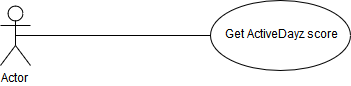
\includegraphics[scale=0.5]{./DiagramsAzhar/Beacon.png}\\\\
\textbf{Pre-condition: }   \\
\begin{itemize}
	\item User need to be registered as Multiply application user.
	\item The user must have a Internet connection.
\end{itemize}
\begin{center}
	\begin{tabular}{ |p{8cm}|p{8cm}| }
		\hline
		\textbf{Actor:} User & \textbf{System:} ActiveDays \\
		\hline
		&  \\
		\hline
		&  \\
		\hline
		& \\   
		\hline
		& \\
		\hline
	\end{tabular}
\end{center}		
\textbf{Post-condition: } \\
\begin{itemize}
	\item 
\end{itemize}
\textbf{Administrator functionality}\\\\
\textbf{UC6 Beacon Registration} \\\\
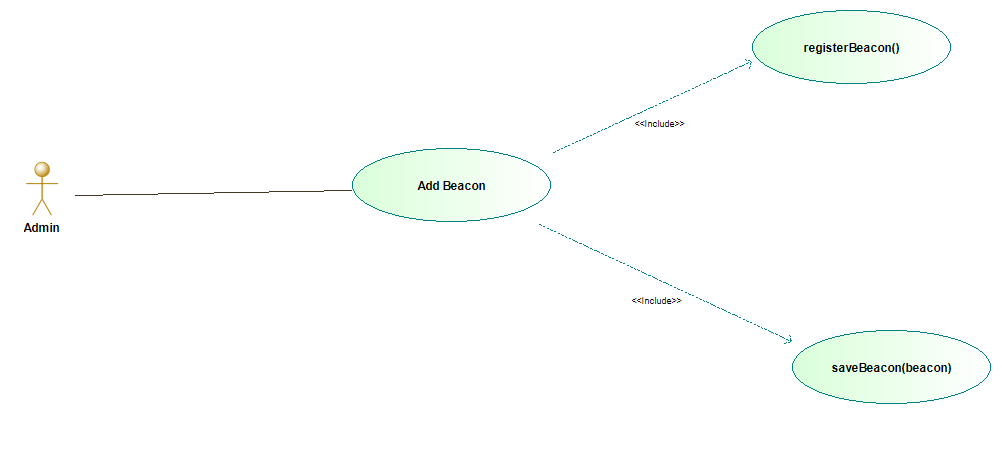
\includegraphics[scale=0.5]{./DiagramsTshepo/addBeacon.png}\\
\textbf{Pre-condition: }   \\
\begin{itemize}
	\item User needs to be registered as an Administrator.
	\item Administrator needs to know location co-ordinates to insert beacon.
	\item Administrator needs to know the Multiply partner ID.
	\item The Administrator must have a Internet connection.
\end{itemize}
\begin{center}
	\begin{tabular}{ |p{8cm}|p{8cm}| }
		\hline
		\textbf{Actor:} User & \textbf{System:} ActiveDays \\
		\hline
		&  \\
		\hline
		&  \\
		\hline
		& \\   
		\hline
		& \\
		\hline
	\end{tabular}
\end{center}		
\textbf{Post-condition: } \\
\begin{itemize}
	\item 
\end{itemize}
\textbf{UC7 Edit Beacon}\\\\
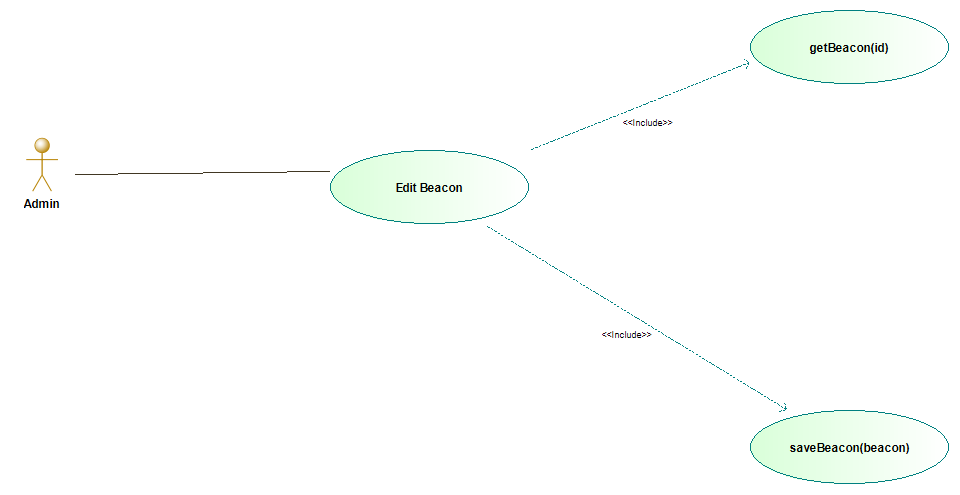
\includegraphics[scale=0.5]{./DiagramsTshepo/editBeacon.png}\\\\
\textbf{Pre-condition: }   \\
\begin{itemize}
	\item User needs to be registered as an Administrator.
	\item Administrator needs to know the location of the beacon, or a property to allow searching.
\end{itemize}
\begin{center}
	\begin{tabular}{ |p{8cm}|p{8cm}| }
		\hline
		\textbf{Actor:} User & \textbf{System:} ActiveDays \\
		\hline
		&  \\
		\hline
		&  \\
		\hline
		& \\   
		\hline
		& \\
		\hline
	\end{tabular}
\end{center}		
\textbf{Post-condition: } \\
\begin{itemize}
	\item 
\end{itemize}
\textbf{UC8 Beacon removal} \\\\
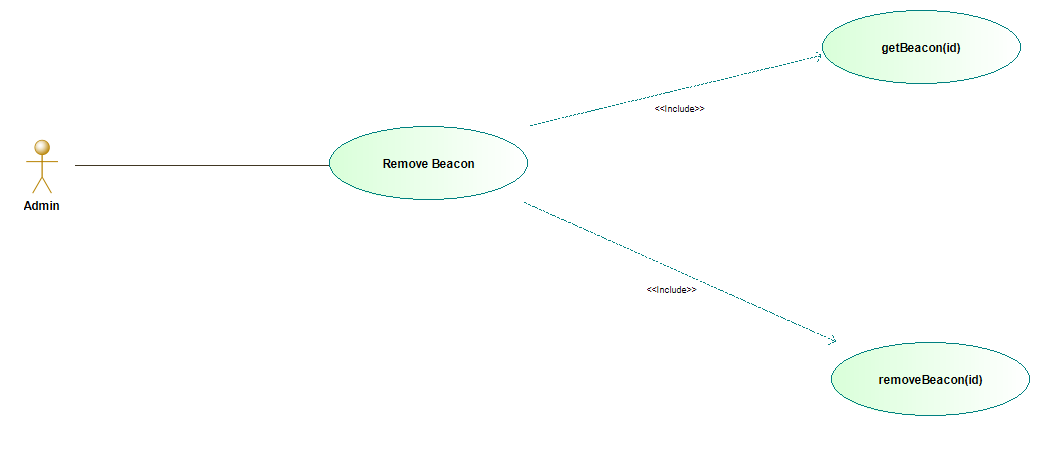
\includegraphics[scale=0.5]{./DiagramsTshepo/removeBeacon.png}\\\\
\textbf{Pre-condition: }   \\
\begin{itemize}
	\item User needs to be registered as an Administrator.
	\item \item Administrator needs to know user id or a user property to allow searching. 
\end{itemize}
\begin{center}
	\begin{tabular}{ |p{8cm}|p{8cm}| }
		\hline
		\textbf{Actor:} User & \textbf{System:} ActiveDays \\
		\hline
		&  \\
		\hline
		&  \\
		\hline
		& \\   
		\hline
		& \\
		\hline
	\end{tabular}
\end{center}		
\textbf{Post-condition: } \\
\begin{itemize}
	\item 
\end{itemize}
\textbf{UC9 Add User}\\\\
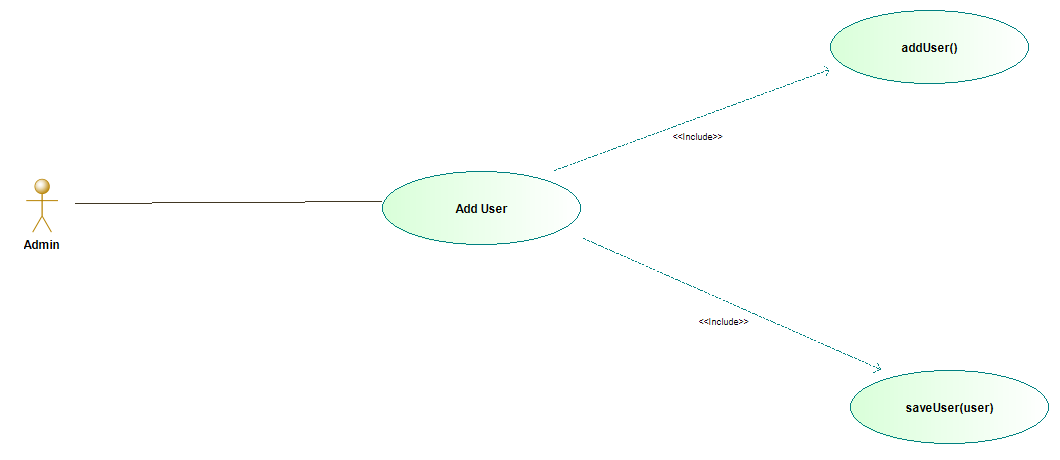
\includegraphics[scale=0.5]{./DiagramsTshepo/addUser.png}\\\\
\textbf{Pre-condition: }   \\
\begin{itemize}
	\item User needs to be registered as an Administrator.
	\item Administrator needs to know user id or a user property to allow searching. 
\end{itemize}
\begin{center}
	\begin{tabular}{ |p{8cm}|p{8cm}| }
		\hline
		\textbf{Actor:} User & \textbf{System:} ActiveDays \\
		\hline
		&  \\
		\hline
		&  \\
		\hline
		& \\   
		\hline
		& \\
		\hline
	\end{tabular}
\end{center}		
\textbf{Post-condition: } \\
\begin{itemize}
	\item 
\end{itemize}
\textbf{UC10 Remove User}\\\\
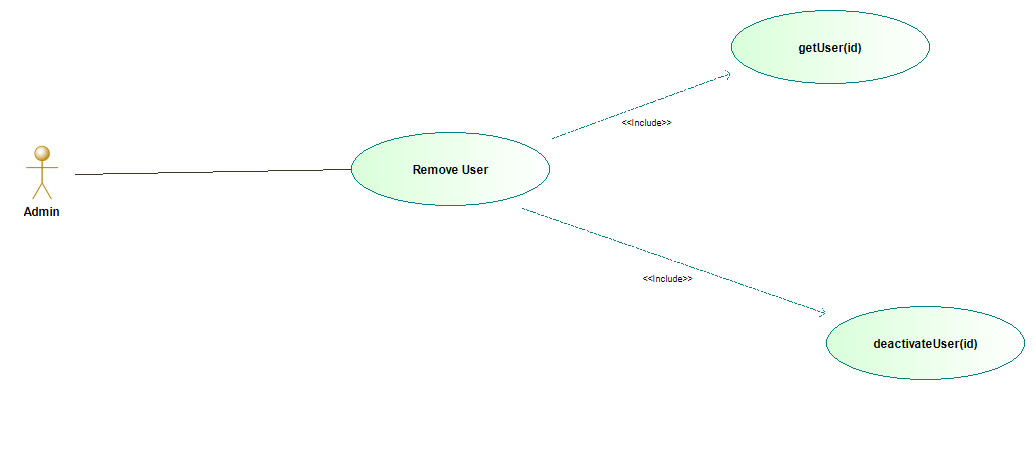
\includegraphics[scale=0.5]{./DiagramsTshepo/removeUser.png}\\\\
\textbf{Pre-condition: }   \\
\begin{itemize}
	\item User needs to be registered as an Administrator.
	\item Administrator needs to know user id or a user property to allow searching. 
\end{itemize}
\begin{center}
	\begin{tabular}{ |p{8cm}|p{8cm}| }
		\hline
		\textbf{Actor:} User & \textbf{System:} ActiveDays \\
		\hline
		&  \\
		\hline
		&  \\
		\hline
		& \\   
		\hline
		& \\
		\hline
	\end{tabular}
\end{center}		
\textbf{Post-condition: } \\
\begin{itemize}
	\item The user will be deactivated from using the application.
\end{itemize}
\textbf{UC11  Edit User}\\
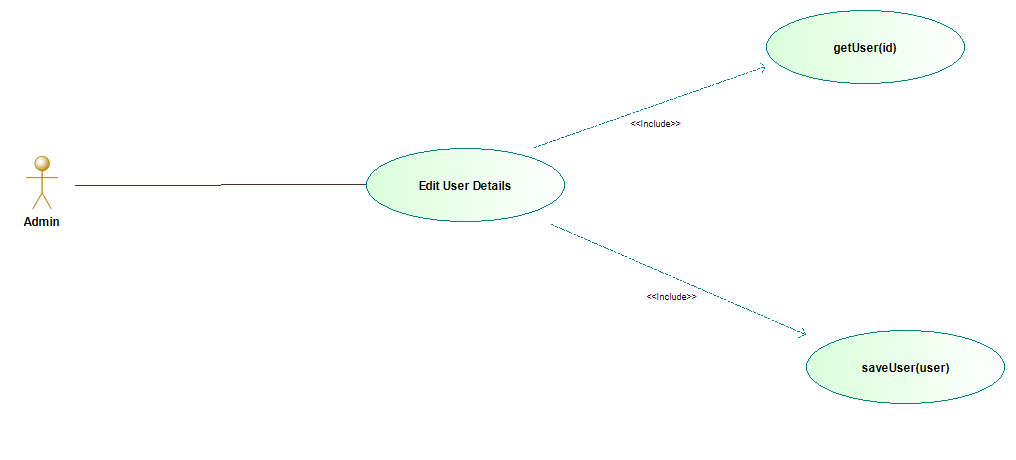
\includegraphics[scale=0.5]{./DiagramsTshepo/editUser.png}\\\\
\textbf{Pre-condition: }   \\
\begin{itemize}
	\item User needs to be registered as an Administrator.
	\item Administrator needs to know user id or a user property to allow searching. 
\end{itemize}
\begin{center}
	\begin{tabular}{ |p{8cm}|p{8cm}| }
		\hline
		\textbf{Actor:} User & \textbf{System:} ActiveDays \\
		\hline
		&  \\
		\hline
		&  \\
		\hline
		& \\   
		\hline
		& \\
		\hline
	\end{tabular}
\end{center}		
\textbf{Post-condition: } \\
\begin{itemize}
	\item After editing and saving user details will be stored back to the system database
\end{itemize}

\subsection{Performance Requirements}

\subsection{Design Constraints}
\textbf{DC1}The mobile application needs a Internet access, and if the 
\subsubsection{Software System Attributes}
\subsubsection{Performance}
The mobile application has to run smoothly, but certain function are dependent on the mobile Internet provider. The server side of the system has to be stable and responsive enough to handle the request from the large user base of Multiply without lagging, that is the server side system's response time must prove to be exceptional no matter the work.
\subsubsection{Flexibility}
The the overall system will consist of a web portal and a mobile application. The mobile application should be able to run on all android devices with the exceptions for Samsung, the mobile application must also support previous versions of android. The administrative portal will be accessible through a browser and can be accessed through any browser.
\subsubsection{Memorability}
Users of the system should be able to remember and navigate the system after the first couple of uses, all user functions, buttons and   
\subsubsection{Usability}
The mobile application should be feel like a natural android application experience and should be simple enough for the user to grasp without to much help. The system must have basic instructions that could be made available to the user by a help button perhaps in the mobile application. Everything should be well displayed in order to better user navigation, the reduction of scrolling is an example.
\subsubsection{Cost}
The cost inquired for this system will be for the server hosting, and the physical beacons.\\
The server hosting will be done on the Amazon AWS-EC2 which is a paid service, the beacons have to be purchased at any retail store that sells them at a good price.

\subsubsection{Integrability}
The system should be easy to integrate. The different parts of the system such as the mobile application and web portal should be able   
\subsubsection{Reliability}
Reliability for this application to work as intended is crucial to its success. If users wish to access the mobile application the user must be always able to access the application. Reliability includes keeping track of user authority, the system should not lose track of what actions each user can perform on the system. Administrators must be able to oversee all the user activity.
\subsubsection{Availability}
The mobile application will be available on the Google play store and can be downloaded by anyone with a mobile application, this will help get the application to all potential users will n android mobile device. The administrative web portal should be accessible inside Multiply, later it might be accessible outside the network of Multiply.
\subsubsection{Security}
The most important security measure is to ensure that Multiply members can register for the mobile application and may be the only individuals that may access the application. They will either set their own user names and passwords or use their Multiply access details which are the user name and password.
In cases where the user has forgotten their password, my group and I decided that an email containing a link should be sent out to a user directing them to a page whereby they will be able to set a new password. If a user fails to get the password correct more than three times in a row, they should be suspended from the application, this will be in use if the user doesn't choose to stay logged into the application. The user is also given the right to suspend their application by discontinuing the application. Once the users have registered and logged in, they will be on a secure line where they can request data regarding their profiles, for security measures the user's authentication details will be sent with the request to ensure all action of the users are authorized. The system also has a administrative web portal, the main goal for this is ensure that the Multiply staff acting as administrators can successfully get authentication using their Multiply access details. Once authenticated the administrator will have access to varies functions that will be granted based on the credentials used to access the web interface.  
\subsubsection{Maintainability}
The maintainability of the application will be managed by Multiply staff after it has been developed by Team Panda Inc, the system has to be well documented and structured n such a way that new developers can easily grasp the system.
\subsection{Other Requirements}
\end{document}
